\section{Running the examples}

\subsection{Running a single iteration}

\begin{frame}[fragile]
\frametitle{Running the examples}
\framesubtitle{Running a single iteration}
\begin{columns}[T]

\column{7cm}

\begin{itemize}
  \item 100 Agents from link 1 to 20
  \item Later from link 20 to 1
  \item Have a look at equil\_plans.xml
  \item Run \verb|org.matsim.run.Controler| with argument \verb|examples/tutorial/| \verb|singleIteration.xml|
  \item Examine the log for errors
\end{itemize}

\column{5cm}
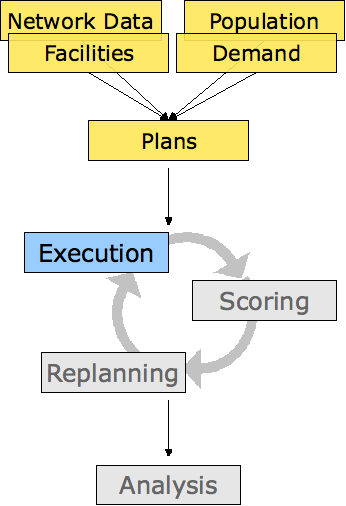
\includegraphics[width=4cm]{../graphics/overviewMatsimExecution.png}

\end{columns}

\end{frame}

\subsection{Visualizing the simulation results}

\begin{frame}[fragile]
\frametitle{Running the examples}
\framesubtitle{Visualizing the simulation results}
\begin{itemize}
  \item Start Netvis again
  \item Open file \verb|output/ITERS/it.0/SnapshotCONFIG.vis|
  \item Change daytime to 06:00 o'clock
  \item Increase linewidth
  \item Press play
  \item Read corresponding events at \verb|output/ITERS/it.0/0.events.txt|
\end{itemize}
\end{frame}


\subsection{Modifying the settings}

\begin{frame}[fragile]
\frametitle{Running the examples}
\framesubtitle{Modifying the settings}

\begin{itemize}
  \item Open \verb|examples/tutorial/singleIteration.xml|
  \item Try to change settings in the module simulation, e.g. endTime of 07:00 or snapshotperiod
  \item Run the simulation again
  \item Be aware of the error: \verb|The simulation will not overwrite files|
  \item Make snapshots in ``googleearth'' mode
\end{itemize}
\end{frame}


\subsection{Running multiple iterations}

\begin{frame}[fragile]
\frametitle{Running the examples}
\framesubtitle{Running multiple iterations}

\begin{columns}[T]

\column{7cm}

\begin{itemize}
  \item Use configuration \verb|examples/tutorial/multipleIterations.xml|
  \item Run controler
  \item 10 Iterations run with 10 \%  agents replanning
  \item Take a look at results
  \item Compare configuration files
  \item Increase number of iterations
\end{itemize}

\column{5cm}
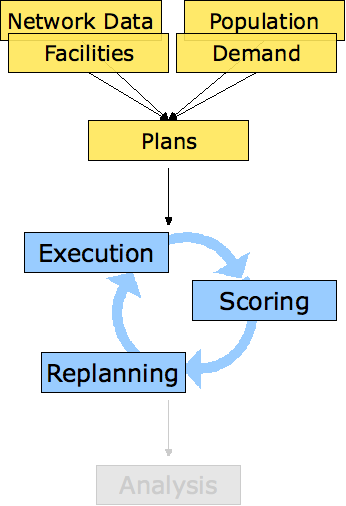
\includegraphics[width=4cm]{../graphics/overviewMatsimIterations.png}

\end{columns}

\end{frame}

\subsection{Modifying the re--planning}

\begin{frame}[fragile]
\frametitle{Running the examples}
\framesubtitle{Modifying the re--planning}

\begin{columns}[T]

\column{7cm}

\begin{itemize}
  \item Change \verb|ModuleProbability_2| in \verb|multipleIterations.xml| to 0.9
  \item Change \verb|ModuleProbability_1| to 0.1
  \item Run simulation again and look at results
  \item Replace value of \verb|Module_2| with \verb|TimeAllocationMutator|
  \item Examine results
  \item Combine the 3 re--routing strategies
\end{itemize}

\column{5cm}
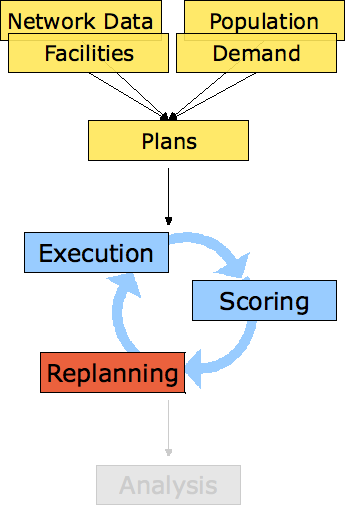
\includegraphics[width=4cm]{../graphics/overviewMatsimReplanning.png}

\end{columns}

\end{frame}
